\section{Generative surface model}
\label{sec:bsm}

\begin{figure*}[t!]
\centering
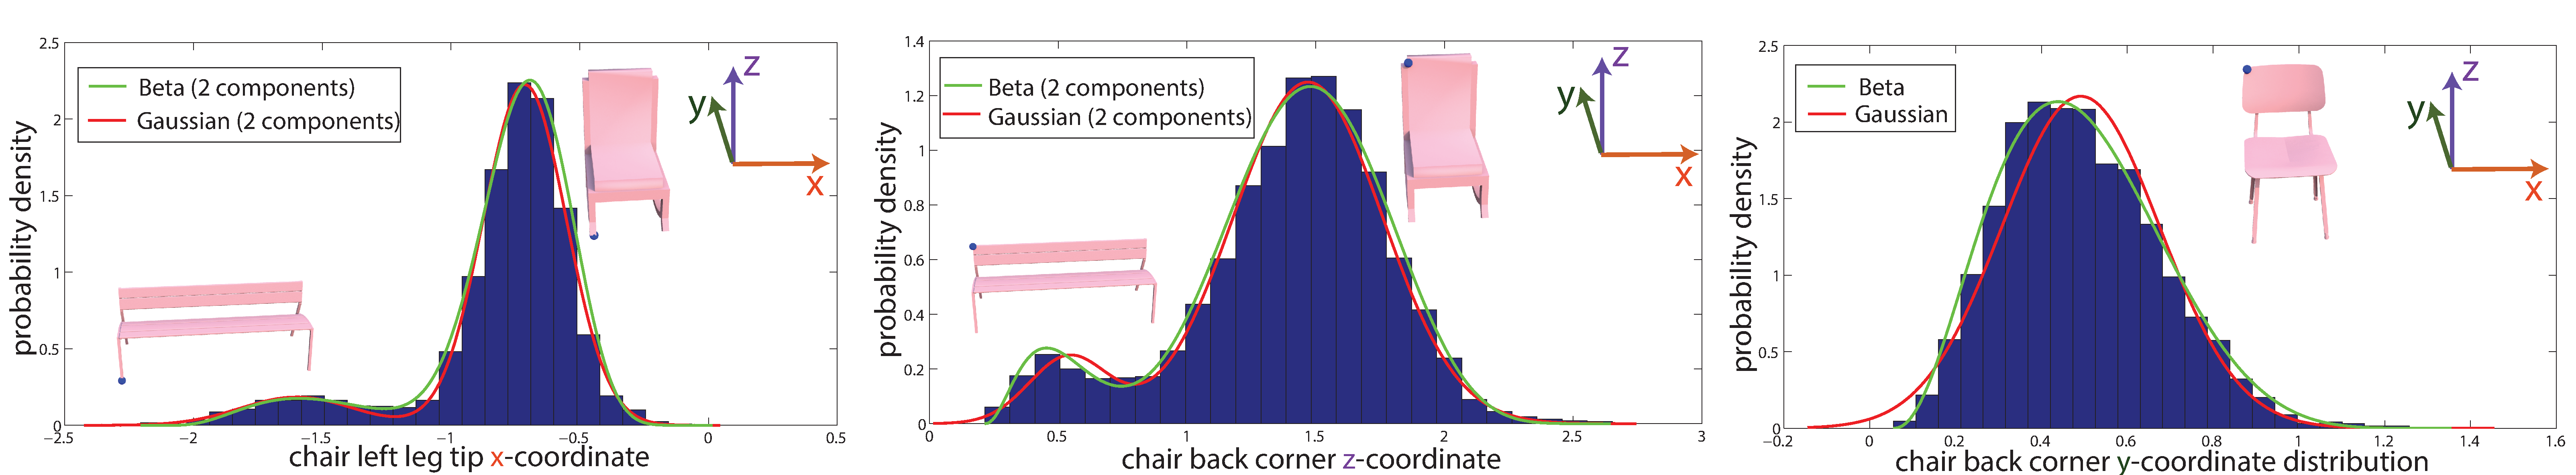
\includegraphics[width=0.95\textwidth]{figures/figure_histograms.pdf}
\vskip -2mm
\caption{Examples of feature point coordinate histograms for chairs and fitted distributions. The fitted Beta distributions are bounded by the minimum and maximum values of the coordinates and fit the underlying probability density more accurately.}
\vskip -8mm
\label{fig:motivation}
\end{figure*}


We now describe a generative probabilistic model whose goal is to characterize surface variability within a shape family. This model is built on the probabilistic shape correspondences and segmentations estimated with the technique described in the previous section. Learning a model that characterizes surface variability poses significant challenges. First, even if we consider individual corresponding surface points, there is no simple probability distribution that can model the variability in their position. For example, Figure \ref{fig:motivation} shows the distributions over coordinates of characteristic feature points across the shapes of four-legged chairs. The coordinates are expressed in an object-centered coordinate system whose origin is located on the chairs' center of mass. We observe that (a) the distributions are not unimodal (Figure \ref{fig:motivation}, left and middle), (b) the modes usually correspond to different types of chairs, such as benches or single-person chairs, and similar modes appear for different feature points (Figure \ref{fig:motivation}, left and middle), (c) even if the distributions appear to be unimodal, they might not be captured with commonly used symmetric distributions, such as Gaussians (red curves). For example, a Gaussian distribution would assign noticeable probability density for unrealistic chairs whose back would be aligned with the center of mass, or is in front of it (with respect to the frontal viewpoint used to display the chairs in the above figure). Furthermore, there are important correlations in the positions of different corresponding points that would need to be captured by the generative model: for example, benches are usually associated with wide seats, short backs, and legs placed on the seat corners. Another complication is that shapes vary in structure: for example, some chairs have armrests, while some others do not. The existence of parts depends on the overall type of chairs. Thus, a generative model needs to capture such structural relationships between parts, as well as capture the dependencies of point positions conditioned on the existence of these parts in the input shapes. Finally, even if our 3D shapes are parameterized with a relatively moderate number of consistently localized points (about $5000$ points), the dimensionality of our input data is still very large ($15000$), which also needs to be handled by the learning procedure of our generative model. \rev{Following the literature in deep learning, the key idea is to design the generative model such that it capture interactions in the surface data hierarchically through multiple layers of latent variables. We experimented with different numbers of hidden layers, and discuss performance differences in Section \ref{sec:results_applications}.} Our surface variability model is defined over the following set of random variables:
\begin{description}[leftmargin=1em]
\setlength{\itemsep}{4pt}
\setlength{\parskip}{0pt}
\setlength{\parsep}{0pt}
\item[Surface point positions] $\bD = \{\bD_{k}\}$ where $\bD_{k} \in \mathbb{R}^3$ represents the position of a consistently localized point $k$ on an input shape expressed in object-centered coordinates. During the training of our model, these random variables are observed by using the inference procedure of the previous section i.e., they are given by the \rev{part template} deformations per input shape. We note that we drop the shape index $t$ since this variable is common across all shapes for our generative model. 
\item[Surface point existences] $\bE = \{\bE_{k}\}$ where $\bE_{k} \in \{0,1\}$ represents whether a point $k$ exists on an input shape. These variables are also observed during training the model of surface variability. They are determined by the inference procedure of the previous section based on which \rev{part templates} were active or inactive per input shape. 
\item[Latent variables for geometry] $\bH = \{H_m^{(1)},H_n^{(2)},H_o^{(3)}\}$ encode relationships of surface point location coordinates at different hierarchical levels. The super-script is an index for the different hidden layers in our model. 
\item[Latent variables for structure] $\bG = \{G_r\}$ encode structural relationships of parts existence in shapes.
\end{description}

\textbf{Model structure.} The generative model is defined through factors that express the interaction degree between the above variables.  The choice of the factors was motivated by experimentation and empirical observations. We start our discussion with the factors involving the observed surface point position variables. Given that these are continuously values variables, one way to model the distribution over point positions would be to use Gaussian distributions. However, as shown in Figure \ref{fig:motivation}, a Gaussian may incorrectly capture the variability even for a single surface point position. Instead, we use Beta distributions that bound the range of values for a variable, and whose density function is more flexible. 
%\begin{wrapfigure}{l}{0.4\columnwidth}
%  \begin{center}
%  \vspace{-10pt}
%    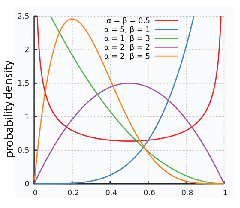
\includegraphics[width=0.5\columnwidth]{figures/beta.pdf}
%\vspace{-10pt}    
%  \end{center}
%\vspace{-10pt}  
%  \caption{Beta distributions}
%\vspace{-10pt}    
%  \label{fig:beta}
%\end{wrapfigure}
The Beta distribution over a single coordinate of an individual point location is defined as follows:
\begin{equation*}
P( D_{k,\tau} ) = \frac{1}{B} D_{k,\tau}^{a-1} \cdot (1 - D_{k,\tau})^{b-1}
\end{equation*}
where the index $\tau=1,2,3$ refers to the x-,y-, or z-coordinate of the point respectively, $B$ is a normalization factor, $a$, $b$ are positive-valued parameters that control the shape of the distribution. The distribution is defined over the interval $[0, 1]$, thus in our implementation we normalize all the observed coordinate values within this range. As discussed above, using a single distribution to capture the statistical variability of a point location is still inadequate since the point locations on a surface are not independent of each other. As shown in Figure \ref{fig:motivation}, the locations are multi-modal and modes are shared, thus we use latent variables to capture these common modes. Putting these empirical observations together, the interaction between point locations and latent variables can be modeled as follows: 
\begin{align*}
& \phi( \bD, \bH^{(1)}) = 
\nonumber \\
& \,\, \prod \limits_{k,\tau} D_{k,\tau}^{a_{k,\tau,0}-1} \cdot (1 - D_{k,\tau})^{b_{k,\tau,0}-1} 
\nonumber \\
& \cdot \prod \limits_{k,\tau} \prod\limits_{m \in \mN_k} D_{k,\tau}^{a_{k,\tau,m} H_m^{(1)}} \cdot (1 - D_{k,\tau})^{b_{k,\tau,m} H_m^{(1)}} 
\nonumber \\
& \cdot \prod \limits_{k,\tau} \prod\limits_{m \in \mN_k} D_{k,\tau}^{c_{k,\tau,m} (1-H_m^{(1)})} \cdot (1 - D_{k,\tau})^{d_{k,\tau,m} (1-H_m^{(1)})}
\end{align*}
where $a_{k,\tau,m}, b_{k,\tau,m},c_{k,\tau,m},d_{k,\tau,m}$ are positive weights expressing how strong is the interaction  between each latent variable $m$ with point $k$, $a_{k,\tau,0}, b_{k,\tau,0}$ are positive bias weights, $\mN_k$ denotes the subset of latent random variables of the first layer connected to the variable $D_k$. To decrease the number of parameters and enforce some sparsity in the model, we split the latent variables in the first layer into groups, where each group corresponds to a semantic part. We model the interaction between each point position with the first hidden layer variables that correspond to the semantic part it belongs to (see also Figure \ref{fig:graphical_model} for a graphical representation of our model). In this manner, each latent variable of the first layer can be thought of as performing a spatially sensitive convolution on the input points per part (see also supplementary material for the inference equations indicating this convolution).

As shown in Figure \ref{fig:motivation}, each group of shapes has its own distinctive parts e.g., benches are associated with wide and short backs. The latent variables of the second layer mediate the inter-dependencies of the part-level latent variables of the first layer. The choice of factors for those interactions are based on sigmoid functions that ``activate'' part-level geometry modes given certain global shape variability modes: 
\begin{align*}
\phi( \bH^{(1)}, \bH^{(2)} ) = \exp \bigg\{ \sum\limits_m w_{m, 0} H_m^{(1)} & + \sum\limits_{m,n} w_{m, n} H_m^{(1)} H_n^{(2)} \nonumber \\ 
& + \sum\limits_n w_{n, 0} H_n^{(2)} \bigg\}
\end{align*}
where the parameters $w_{m,n}$ control the amount of interaction between the latent variables of the first and second layer, $w_{m, 0}$, $w_{n, 0}$ are bias weights. Given the above factor, it can be seen that each latent variable is activated through sigmoid functions:
\begin{align*}
P( H_m^{(1)} = 1 | \bH^{(2)} ) = \sigma ( w_{m, 0} + \sum\limits_{n} w_{m, n} H_n^{(2)} ) \\
P( H_n^{(2)} = 1 | \bH^{(1)} ) = \sigma ( w_{n, 0} + \sum\limits_{m} w_{m, n} H_m^{(1)} ) 
\end{align*}
where $\sigma(x)=1/(1+exp(-x))$ represents the sigmoid function. 


\begin{figure}[t!]
\includegraphics[width=1.0\columnwidth]{figures/dbm}
\vskip -2mm
\caption{Graphical representation of the surface variability model based on our airplane dataset.}
\label{fig:graphical_model}
\vskip -8mm
\end{figure}


We model the interactions of the latent variables of the subsequent hidden layers in the same manner.  By multiplying all of the above factors, we combine them into a single probability distribution, which has the form of a deep Boltzmann machine \cite{Salakhutdinov12}. By taking into account that some factors must be deactivated when parts are non-existing in shapes (i.e., when the existence variables for their points are $0$), our final probability distribution has the following form: 
\begin{align}
& P_{bsm}( \bD, \bH, \bG, \bE ) = \frac{1}{Z} \exp \bigg\{ 
\nonumber  \\
& \sum\limits_{k,\tau} (a_{k,\tau,0}-1) \ln(D_{k,\tau})E_k + \sum\limits_{k,\tau} (b_{k,\tau,0}-1) \ln(1-D_{k,\tau})E_k 
\nonumber  \\
& +\sum\limits_{k,\tau,m \in \mN_k} a_{k,\tau,m} \ln(D_{k,\tau}) H_m^{(1)}E_k 
\nonumber  \\
& +\sum\limits_{k,\tau,m \in \mN_k} b_{k,\tau,m} \ln(1-D_{k,\tau}) H_m^{(1)}E_k
\nonumber  \\
& +\sum\limits_{k,\tau,m \in \mN_k} c_{k,\tau,m} \ln(D_{k,\tau}) (1-H_m^{(1)})E_k 
\nonumber  \\
& +\sum\limits_{k,\tau,m \in \mN_k} d_{k,\tau,m} \ln(1-D_{k,\tau}) (1-H_m^{(1)})E_k
\nonumber \\
& +\sum\limits_m w_{m, 0} H_m^{(1)} + \sum\limits_{m,n} w_{m, n} H_m^{(1)} H_n^{(2)} + \sum\limits_n w_{n,0}H_n^{(2)}
\nonumber \\
& + \sum\limits_{n,o} w_{n, o} H_n^{(2)} H_o^{(3)} + \sum\limits_o w_{o, 0} H_o^{(3)} 
\nonumber \\
& +\sum\limits_k w_{k,0} E_k + \sum\limits_{k,r} w_{k, r} E_k G_r + \sum\limits_r w_{r, 0}G_r \bigg\} 
\label{eq:BSM}
\end{align}
where $Z$ is a normalization constant. In the following paragraphs, we refer to this model as Beta Shape Machine (BSM) due to the use of Beta distributions to model  surface data.

\textbf{Parameter learning.} Learning  the parameters of the BSM model poses a number of challenges. Exact maximum likelihood estimation of the parameters is intractable in Deep Boltzmann machines, thus we resort to an approximate learning scheme, called contrastive divergence \cite{Koller09}. Contrastive divergence aims at maximizing the probability gap between the surface data of the input shapes and samples randomly generated by our model. The intuition is that by increasing the probability of the observed data relative to the probability of random samples, the parameters are tuned to model the input data better. The objective function of contrastive divergence is defined as follows: 
\begin{align*}
L_{CD} = \frac{1}{T} \sum\limits_t [ \ln \tilde{P}_{bsm}(\bksi_t) - \ln \tilde{P}_{bsm}(\bksi'_t) ]
\end{align*}
where $T$ is the number of training examples, $\tilde{P}_{bsm}$ is given by Equation \ref{eq:BSM} without the normalization factor $Z$ (known as unnormalized measure), $\bksi_t$ is an assignment to the variables of the model given an input shape $t$ and $\bksi'_t$ is an assignment to the variables according to a sample perturbed from the same input shape $t$. The assignments to the variables $E_k$ and $\bD_k$ per input shape $t$ are set by checking if the \rev{part template} exists in the input shape and finding the closest surface point to each point $k$ on the deformed \rev{part templates} for it respectively. The assignments for the latent variables are computed by performing mean-field inference and using the expectations of their approximating distributions, following Salakhutdinov et al. \cite{Salakhutdinov12} (see supplementary material for more details). The perturbed sample is generated by inferring the approximating probability distribution of the top-layer binary variables given an input shape, then sampling these binary variables according to their distribution, and finally computing the expectations of the approximating distributions of all the other variables in the model given the sampled values of the top layer. 


\begin{figure}[t!]
\centering
\includegraphics[width=0.99\columnwidth]{figures/bsm_sample}
\vskip -2mm
\caption{Samples generated from the BSM for airplanes and chairs. The generated shapes are implicitly segmented into labeled parts since each point is colored according to the label of the \rev{part template} it originated from.}
\vskip -8mm
\label{fig:sample_BSM}
\end{figure}


An additional complication in parameter learning is that even for collections whose shapes are parameterized with a relatively moderate number of points and even with the sparsity in the connections between the observed variables and the first hidden layer, the number of parameters ranges from $5$ to $10$ million. Yet the available organized 3D shape collections are limited in size e.g., the corrections we used contain only a few thousand shapes. A key idea in our learning approach is to use strong spatial priors that favor similar weights on the variables representing point positions that are spatially close to each other on average across the input shapes of our collections. To favor spatial smoothness in the learned parameters, we change the above objective function with the following spatial priors and $L^1$ norm regularization terms. The $L^1$ norm was desired to eliminate weak hidden node associations causing higher noise when sampling the model and also prevent model overfitting. The new objective function is defined as follows:
\begin{align*}
L_{CD,spatial} & = \frac{1}{T} \sum\limits_t [ \ln \tilde{P}_{bsm}(\bksi_t) - \ln \tilde{P}_{bsm}(\bksi'_t) ] 
\nonumber \\
& - \lambda_1 \sum\limits_{k,\tau,k' \in \mN_k,m} | a_{k,\tau,m} - a_{k',\tau,m} | - \lambda_2 \sum\limits_{k,\tau,m} | a_{k,\tau,m} | 
\nonumber \\
& - \lambda_1 \sum\limits_{k,\tau,k' \in \mN_k,m} | b_{k,\tau,m} - b_{k',\tau,m} | - \lambda_2 \sum\limits_{k,\tau,m} | b_{k,\tau,m} | 
\nonumber \\
& - \lambda_1 \sum\limits_{k,\tau,k' \in \mN_k,m} | c_{k,\tau,m} - c_{k',\tau,m} | - \lambda_2 \sum\limits_{k,\tau,m} | c_{k,\tau,m} | 
\nonumber \\
& - \lambda_1 \sum\limits_{k,\tau,k' \in \mN_k,m} | d_{k,\tau,m} - d_{k',\tau,m} | - \lambda_2 \sum\limits_{k,\tau,m} | d_{k,\tau,m} | 
\nonumber \\
& - \lambda_1 \sum\limits_{k,r,k' \in \mN_k} | w_{k,r} - w_{k',r} | 
\nonumber \\
& - \lambda_2( \sum\limits_{m,n} | w_{m,n} | - \sum\limits_{n,o} | w_{n,o} | - \sum\limits_{k,r} | w_{k,r} | ) \\
\end{align*}
where $\lambda_1, \lambda_2$ are regularization parameters, set to $10^{-3}$ and $10^{-4}$ respectively in our experiments, $\mN(k)$ here denotes all the variables representing point positions whose average distance to point $k$ is less than $10\%$ of the largest distance between a pair of points across all shapes. We perform projected gradient ascent to maximize the above objective function under the constraint that the parameters $a_{k,m}, b_{k,m},c_{k,m},d_{k,m}$ are all positive. The same parameters are initialized to random positive numbers according to a uniform distribution on $[10^{-7},10^{-3}]$, while the rest of the weights are initialized according to a normal distribution with mean $0$ and variance $0.1$. 

\begin{figure}[t!]
\centering
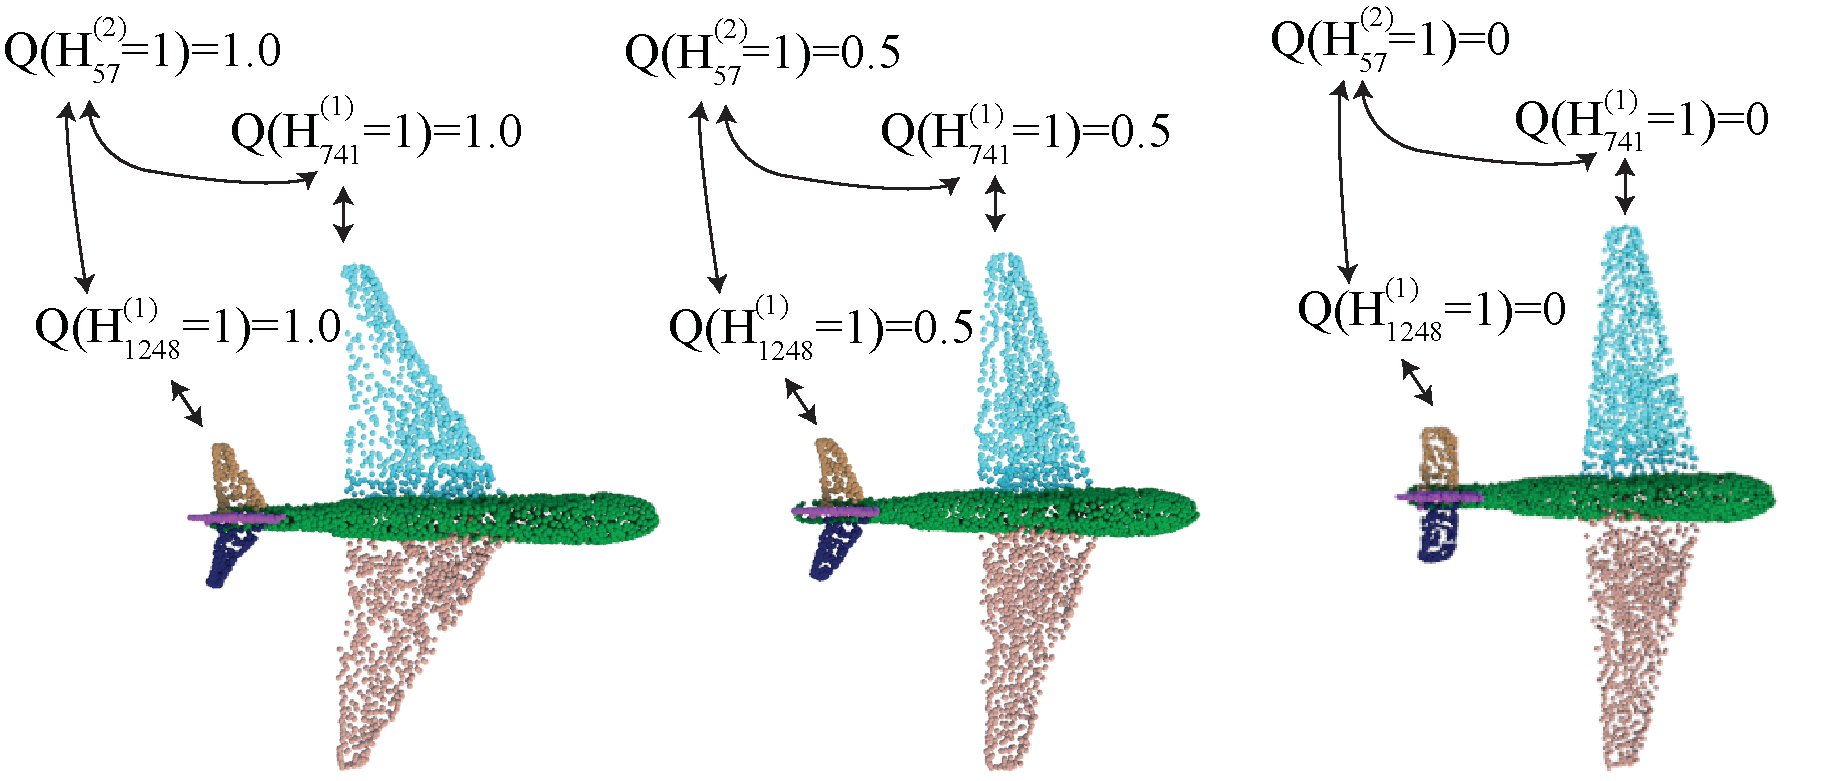
\includegraphics[width=0.9\columnwidth]{figures/motivation/motivation.pdf}
\vskip -3mm
\caption{\rev{Certain latent variables in our learned model have meaningful interpretations.  For example, given the leftmost delta-shaped wing arrangement, certain hidden variables of the first layer are activated (i.e., activation probability based on mean-field inference becomes approximately one), while given the rightmost straight wing arrangement, the same variables are deactivated. Similarly, other first layer variables are activated and deactivated  for triangular and straight tailplanes respectively. The model also learns that there is a potential statistical correlation between straight wings and tailplanes through variables of the second layer. Initializing the synthesis procedure with interpolated probabilities (e.g., 50\%) of these variables generate plausible intermediate configurations of wings and tailplanes (middle).} }
\label{fig:motivation2}
\vskip -8mm
\end{figure}


To avoid local minima during learning, we perform pre-training \cite{Salakhutdinov12}: we first separately train the parameters between the surface points layer and the first hidden layer, then the parameters of the first and second hidden layer, and so on. Then in the end, our method jointly learns the parameters of the model across all layers.  To train our model with contrastive divergence, we also found that it was necessary to apply our training procedure separately on the part of the model involving the interaction parameters between the existence variables $E_k$ and the latent variables $\bG$, then the parameters involved in the rest of the model are learned conditioned on the existence variables $E_k$ \cite{Marlin08}. Otherwise, the parameters of the model were abruptly diverging due to the three-way interaction of the existence variables, point position variables and the first-layer latent variables. For more details regarding learning and parameter update equations, we refer the reader to the supplementary material and provided source code. \rev{Figure \ref{fig:motivation2} demonstrates a characteristic example of the information captured in latent variables of our model after learning. In the results section, we discuss fine-grained classification experiments indicating the relationship of the uppermost layer variables with high-level shape attributes, e.g., shape types.}


\textbf{Number of latent variables.} A significant factor in the design of the model is the number of latent variables $\bG$ and $\bH$. Using too few latent variables in the model results in missing important correlations in the data and causing large reconstruction errors during training. Using too many latent variables causes longer training times, and results in capturing redundant correlations.  We practically experimented with various numbers of latent variables per layer, and checked performance differences in terms of correspondence accuracy (see joint shape analysis and synthesis paragraph).  The best performance was achieved by selecting the number of latent variables of the first layer to be $1/10th$ of the total number of the point position variables $\bD$ per part. The number of latent variables in the second layer was $1/5th$ of the number of latent variables in the first layer, and the number of latent variables in the third layer $\bH^{(3)}$ was $1/2.5th$ the number of latent variables in the second layer. The number of latent variables $\bG$ was set equal to the total number of latent variables $\bH^{(1)}$. 

\textbf{Shape synthesis.} To perform shape synthesis with the generative model, we first sample the binary variables of the top hidden layer, then we alternate twice between top-down and bottom-up mean-field inference in the model. We then compute the expectations of the surface point existences and location variables based on their inferred distributions. The result is a point cloud representing the surface of a new shape. Figure \ref{fig:sample_BSM} shows representative sampled point clouds. The point clouds consists of $5000$ points. Due to the approximate nature of learning and inference on our model, the samples do not lie necessarily on a perfect surface. Due to their low number, we cannot apply a direct surface reconstruction technique. Instead, we find parts in the training shapes whose corresponding points are closest to the sampled point positions based on their average Euclidean distances. Then we apply the embedded deformation method \cite{Sumner:2007:EDS} to preserve the local surface detail of the used mesh parts, and deform them smoothly and conservatively towards the sampled points. A deformation graph of $100$ nodes is constructed per part, and nodes are deformed according to the nearest sampled points. We use the following parameters found in \cite{Sumner:2007:EDS}: $w_{rot}=3$,  $w_{reg}=15$, $w_{con}=120$ and set the deformation node neighborhood size equal to $20$. Figure \ref{fig:synthesis_results} shows synthesized shapes based on the sampled point clouds and the closest training shape parts (in blue). As it can been, the model learns important constraints for generating plausible shapes, such as symmetries and functional part arrangements.



\textbf{Joint shape analysis and synthesis.}
The BSM model can be used as a surface prior to improve shape correspondence. To do this, we combine the deformation model of the previous section and the BSM generative model into a single joint probability distribution, and find the most likely joint assignment to all variables: 
\begin{align*}
\textrm{maximize~~}
P_{crf}( \bY, \bU, \bS, \bD | \bX ) \cdot P_{bsm}( \bD, \bH, \bG, \bE )
\end{align*}
The most likely joint assignment to the above variables is found again with mean-field inference. First, we apply the Algorithm \ref{algorithm} to compute initial correspondences and segmentations, and train the BSM model based on the estimated correspondences and segmentations. Then we perform mean-field inference on the joint model to compute the most likely assignments to all variables based on their inferred approximating distribution modes, yielding improved point correspondences. We alternate between training the BSM model and mean-field inference $3$ times in our experiments, after which we did not notice any considerable improvement.

\begin{figure}[t!]
\centering
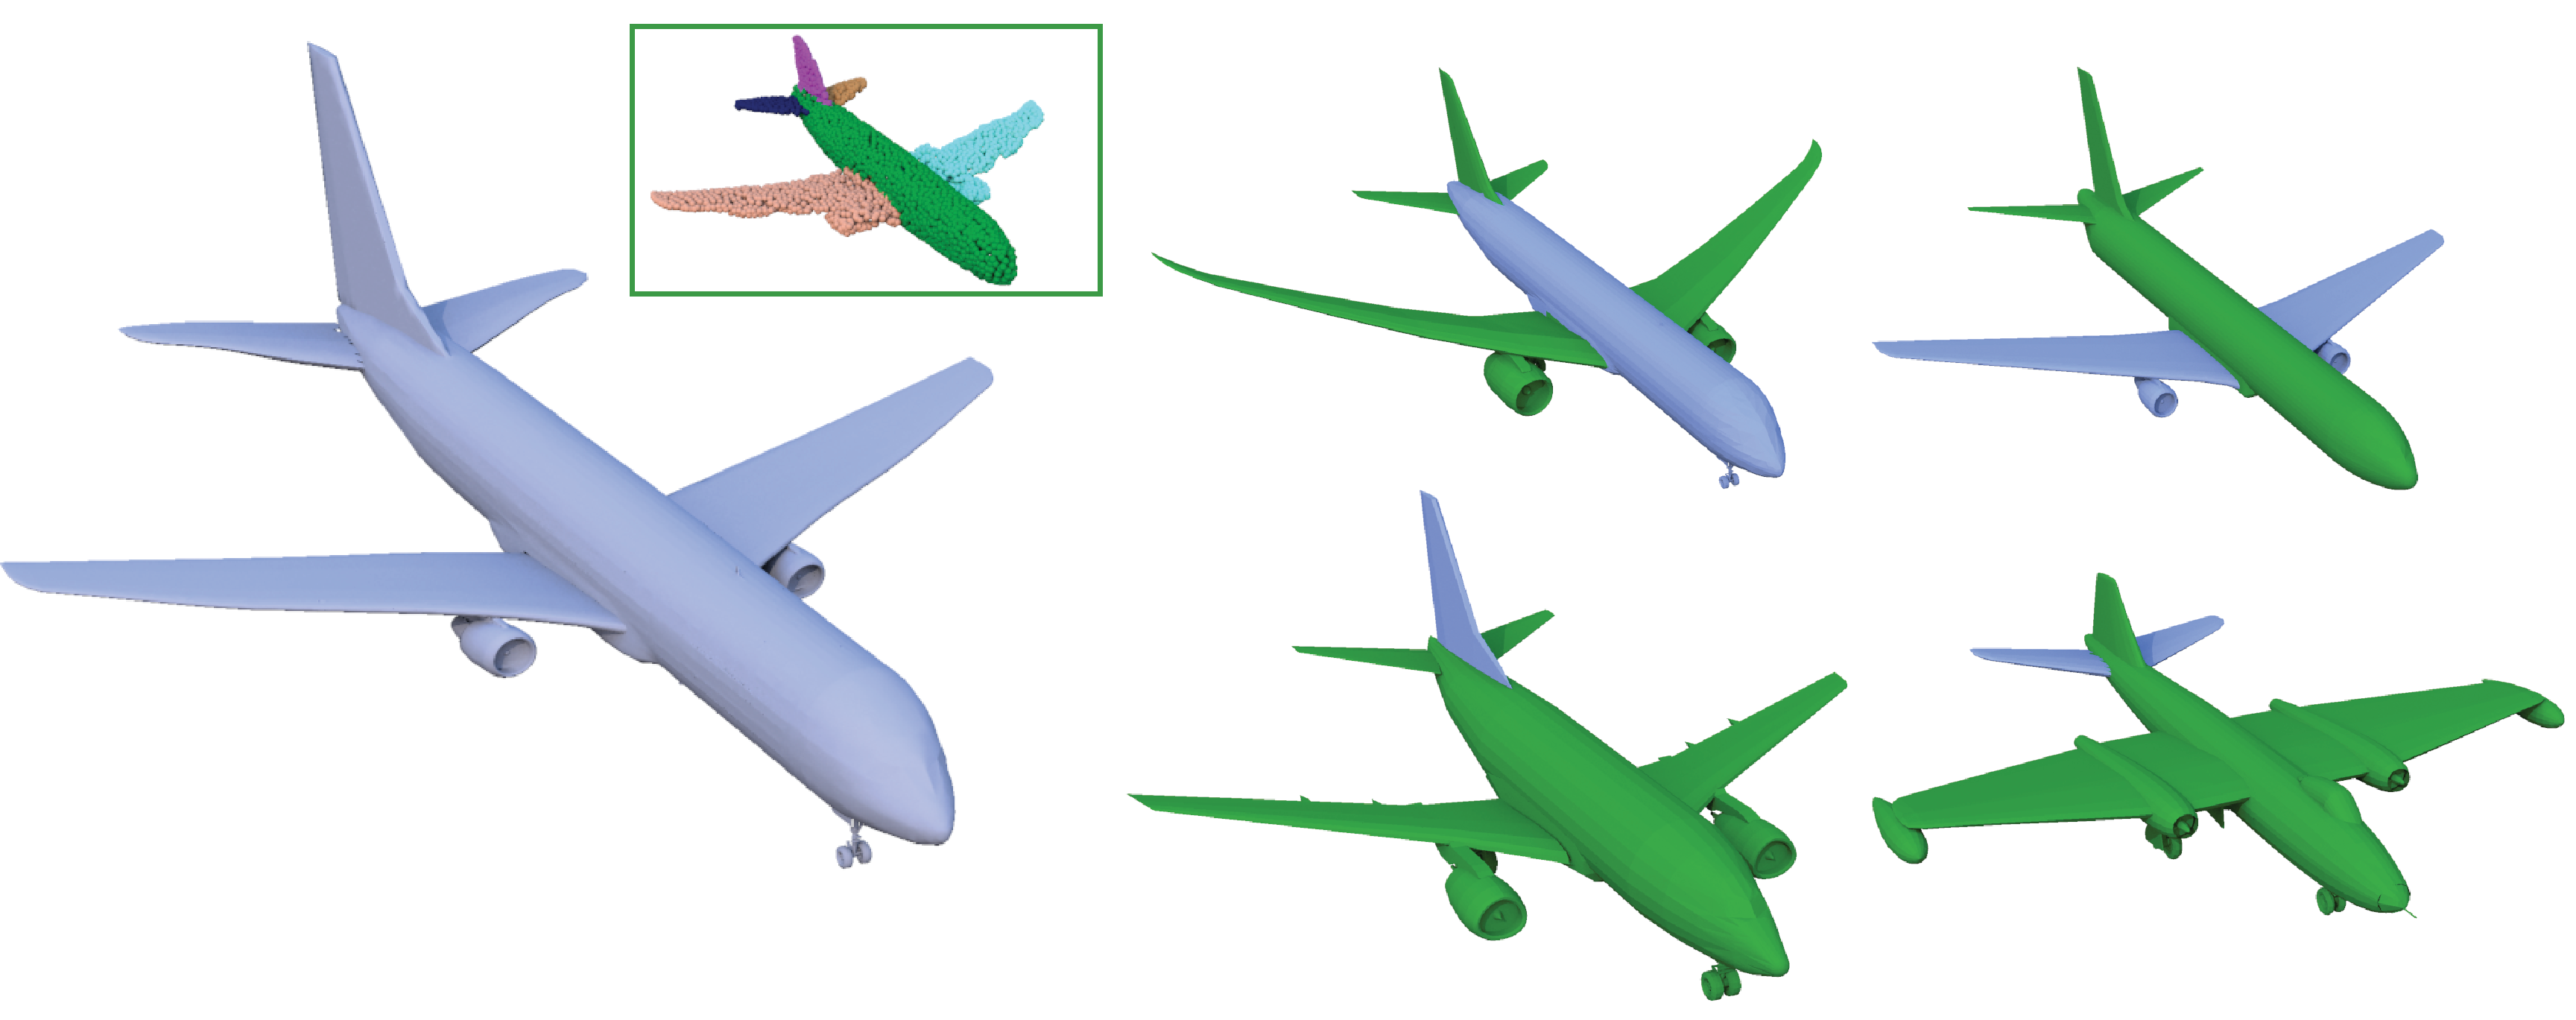
\includegraphics[width=0.83\columnwidth]{figures/synthesis_airplane}
\vskip -1mm
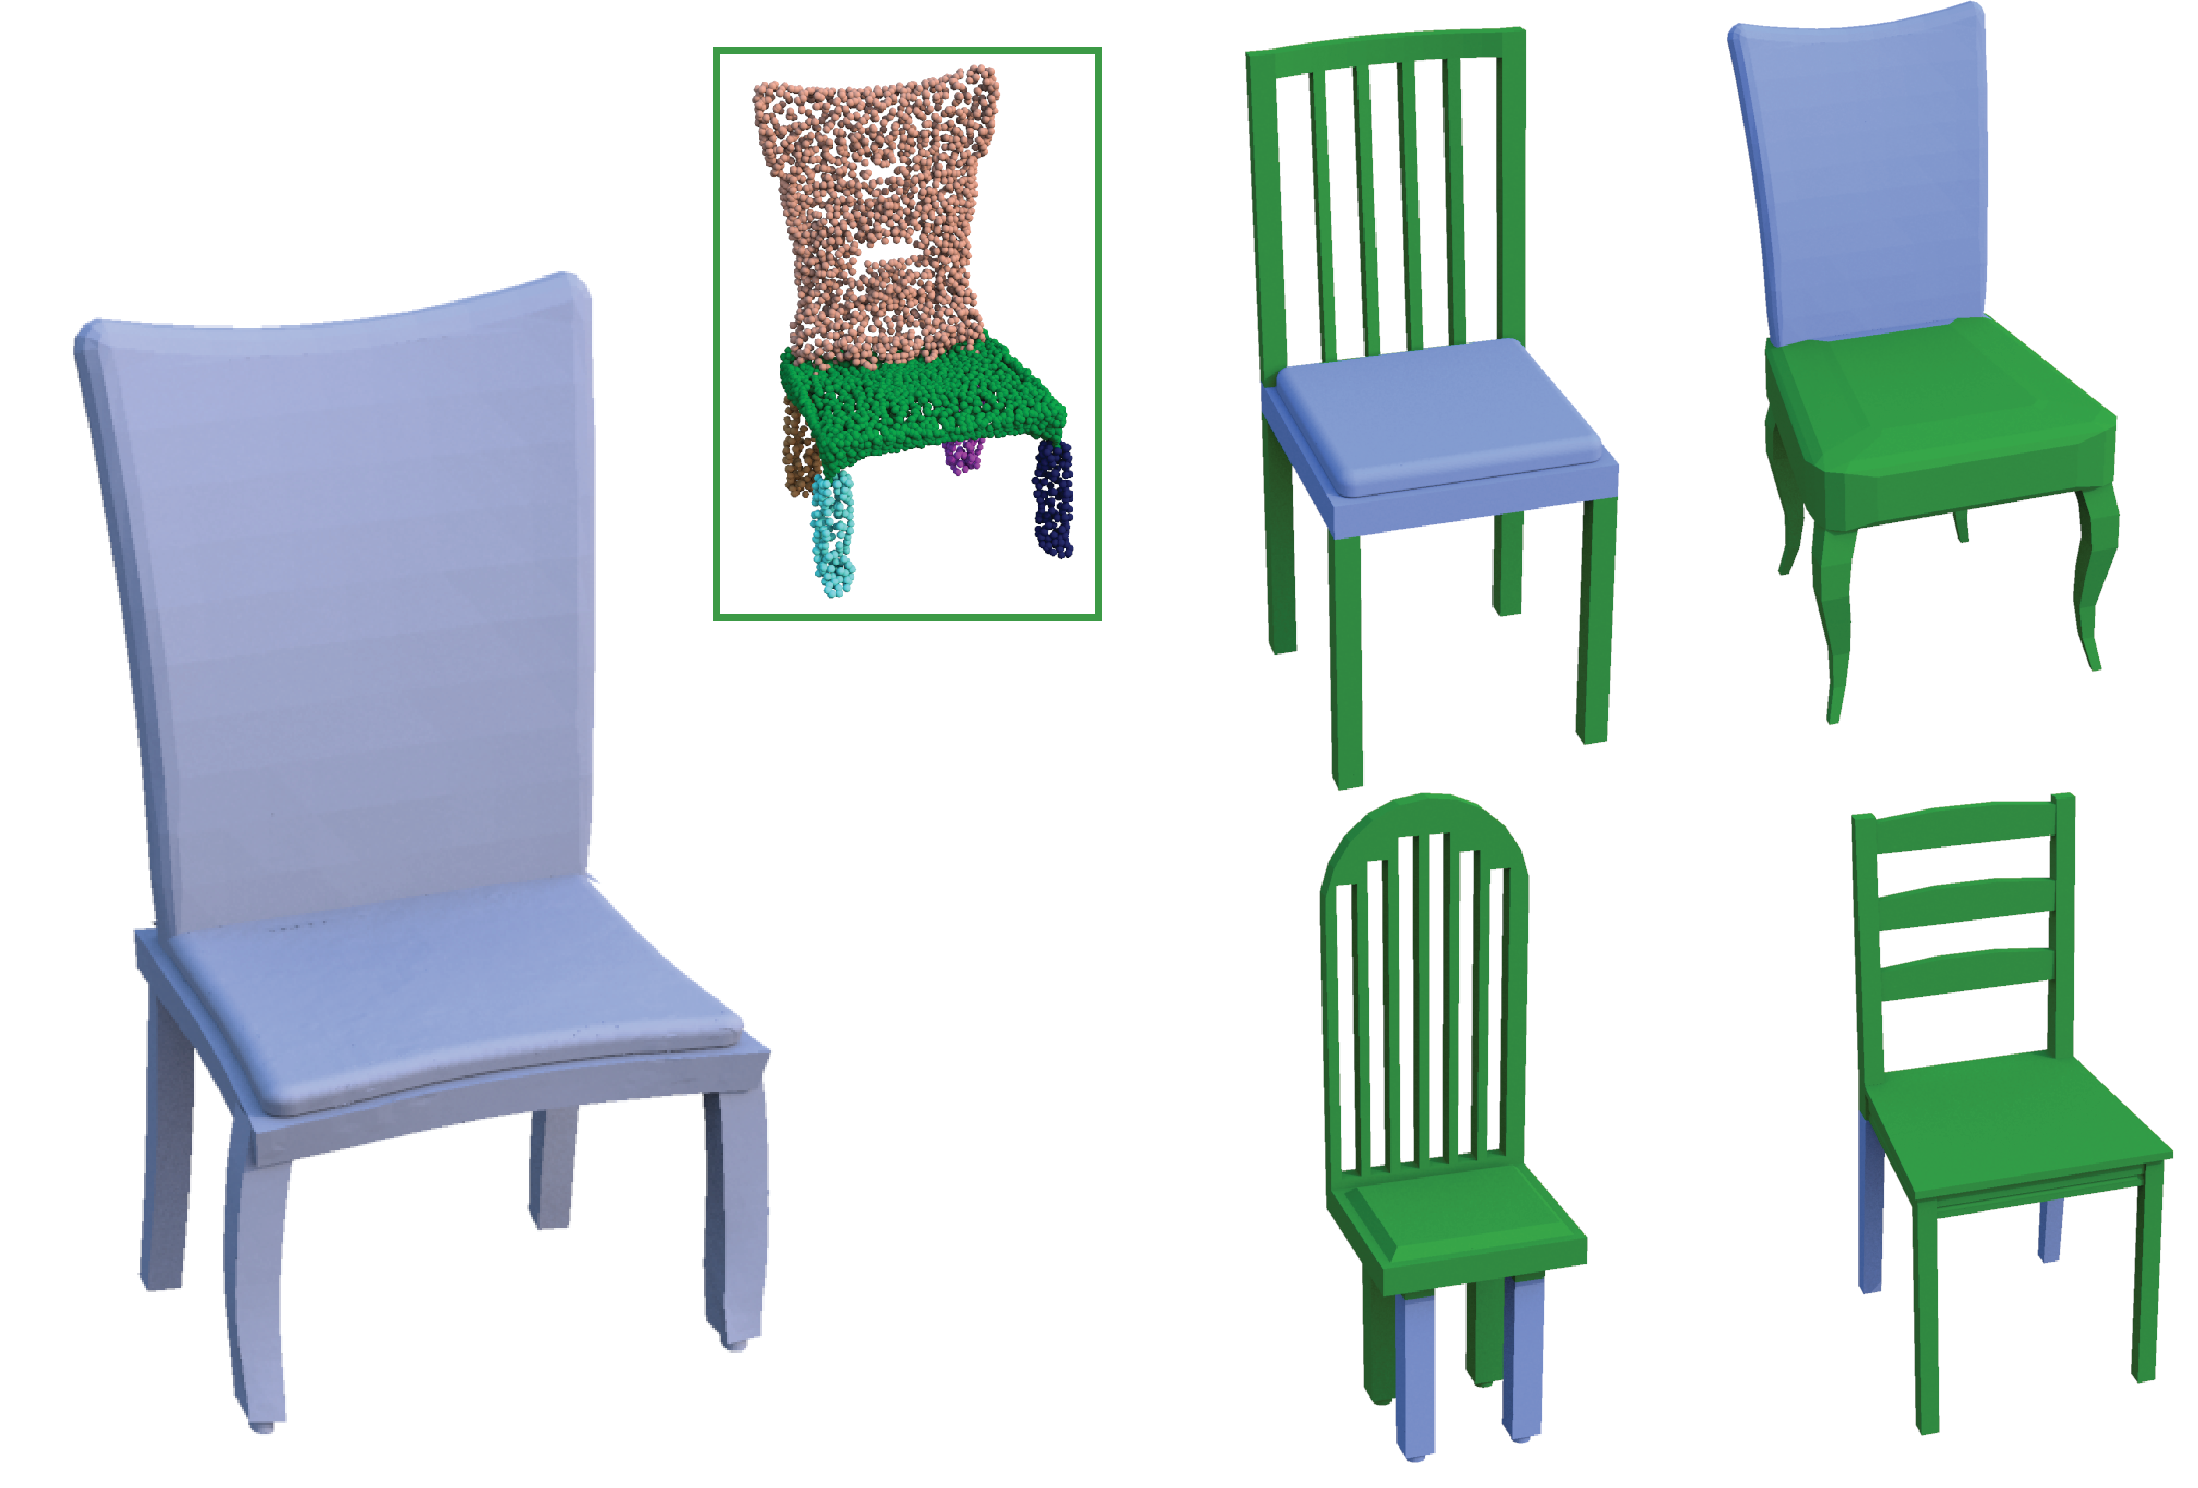
\includegraphics[width=0.83\columnwidth]{figures/synthesis_chair}
\vskip -3mm
\caption{Synthesis of new shapes (left) based on the Beta Shape Machine samples (green box) and embedded deformation on input shape parts (right).}
\vskip -8mm
\label{fig:synthesis_results}
\end{figure}
